\documentclass[pdftex,12pt,letter]{article}
\usepackage{fancyhdr}
\usepackage{enumerate}
\usepackage{tabularx}
\usepackage{graphicx}
\usepackage{caption}
\usepackage{subcaption}
\usepackage{array}
\usepackage[toc,page]{appendix}
\usepackage[justification=justified,singlelinecheck=false]{caption}
\usepackage{placeins}
\usepackage{hyperref}
\usepackage{algorithmic}
\usepackage{algorithm}
\usepackage{amsmath}
\pagestyle{fancy}
\makeatletter
  \renewcommand\@seccntformat[1]{\csname the#1\endcsname.\quad}
\makeatother

\newcolumntype {Y}{ >{\raggedright \arraybackslash }X}
\newcommand{\HRule}{\rule{\linewidth}{0.5mm}}
\captionsetup{labelformat=empty}

\DeclareMathOperator{\length}{length}

\begin{document}

\begin{titlepage}
\begin{flushright}
\HRule \\[0.4cm]
{ \bfseries
{\huge EECS 405 Final Report\\[1cm]}
{\Large for\\[1cm]}
{\large Improving Efficiency of String Similarity Searches through Indexed Pruning\\[3cm]}
{\large Prepared by\\[1cm]James Fitzpatrick\\Kyle Patterson\\[2cm]
Version 1.0\\
May 2, 2014\\
}}
\end{flushright}
\end{titlepage}

\tableofcontents\newpage

\section{Abstract}
Numerous solutions exist to deal with the problems caused by data set inconsistencies, such as k-gram similarity and top-k edit distance. However, many of these solutions are limited by data size, as k-gram computation can be both time and resource intensive. With the decrease in digital storage space cost, the average size of data sets has seen rapid growth in the past decade, and frequently trumps the limitations of existing string similarity solutions. This paper proposes merging the realms of data mining and similarity queries as a valid means of reducing search times in large data sets while maintaining high accuracy in similarity query results.

\section{Introduction}
String similarity search is a rapidly growing area of research within the computer science community due to its numerous overlapping applications in the modern world. From simple database joins to biological queries (such as \textit{'Are these two genes from the same family?'}) to online social presence (\textit{'Do these two accounts belong to the same user'}), being able to identify two objects that are highly similar to each other has proven necessary to understand the current world. \\
\\
With increases in digital storage, the average query space has increased from kilobytes of space to gigabytes and, in some cases, terabytes. This query space can now contain tens of thousands to millions of entries. While exhaustive searching can be conducted in linear time, an exhaustive similarity search would require computing the edit distance between the query and every entry in at-best pseudo-quadratic time, which is no longer feasible with such large data sets.\\
\\
The problem becomes much more prevalant when we consider more advanced similarity search techniques, such as k-edit pruning and k-gram searching. The former prunes the search space by removing the candidate from the search space once known edits reach some threshold $k$, but otherwise operating as an exhaustive search. In k-gram searching, grams of length $k$ are constructed and stored for reference later; words with more than a predefined threshold of grams in common are considered similar and returned. While gram searching is much more efficient than exhaustive search, it is more expensive in overhead as these grams must be constructed and stored, leading to high access cost on query execution.\\
\\
One particular field of computer science, data mining, was established specifically to deal with such large data searching problems, and has produced several techniques that could be helpful in large-scale similarity searching. Cluster analysis, or clustering, 

\section{Problem Definition}
Let S be a complete data set consisting of strings from alphabet $\Sigma$. For each string $s_i$ in S, we define the following:
\begin{itemize}
\item $\length(s_i)$ = number of characters in $s_i$.\\ For example, $\length('run') = 3$.
\item LCS($s_i$,$s_j$) = longest common substring between $s_i$ and $s_j$.\\ For example, LCS('$run$','$fun$') = '$un$'.
\end{itemize}

We define the InvertedList I as follows:

\begin{itemize}
\item For each element $i$ in I, every element of $i$ is either an InvertedList or a string
\item Every InvertedList $i$ in I has a key that equals the longest common substring of all elements in $i$
\end{itemize}

\section{Related Work}
TODO: Merge together literature review

\subsection{String Similarity}

\subsection{Top-K Search}
Top-K Search, a search utilized in String Similarity, computes the top k results by comparing a query string to a dataset and finds the k elements that have the smallest edit distance from this string. However, this algorithm can become computationally expensive as the algorithm requires comparing the query to all strings in a dataset. To reduce the number of necessary computations, we implement a version of the pivotal Top-K Search as described by Deng et al. A trie-based approach can take advantage of the similarity strings. Each entry in the trie represents a character, save the root which is the null character. The path from the root to a leaf is a inorder representation of that string. This structure redcudes the number of strings we need to store in full by taking advantage of strings with similar prefixes. By using this trie, we can incrementally search the entire search space simultaneously utilizing edit distance measurements. Once k strings have been found, we have our strings to return. 

\subsection{Positional VGRAM Search}

Gram based appraoches to string similarity have been discussed for quite some time. By assembling a inverted list of grams, we can divide a query into grams of size n to compare it to the strings of a dataset. The strings that share the most grams with this string should be considered to be "closer" to the query than others. Many string comparison algorithms consider grams of set lengths. However, there are many advantages and disadvantages to having any particular length of n-gram. Rather than to have a one-for-all solution to the strings, the authors propose a solution to generate grams of variable length between a minimum and maximum length based on a set gram dictionary, which is constructed based on the data collection of strings prior to the query. When computing the gram dictionary, we should only store longer grams that have a frequency above a certain threshold. The algorithm utilizes a trie to reduce the computations of grams that are substrings of longer grams, since the subgrams will necessarily occur when the larger grams are present. Since smaller grams are present in larger ones, the grams that survive pruning will more often than not be shorter grams. Longer grams will be present in data sets only if they are very frequent. By this pruning, we can reduce our gram set to the grams that are most helpful in indentifying desired strings. Further, the position of these grams may be of importance to certain datasets. In some sets, a particular gram may occur at the beginning of the ending of a string, which will identify strings more accurately. By adding positional information, we can also reduce our search space. 

\section{Methodology}
\subsection{Data preparation}
Data was mirrored from the Database and Logic Programming bibliography (DBLP) and International Movie Database (IMDB) public sources to a MySQL server hosted on a micro instance of Amazon Elastic Cloud Computing (EC2). Data was cleaned to remove any incomplete entries, and trimmed to remove any entries that contained any non-standard ASCII characters (i.e, characters whose value is greater than 127).\\
\\
In total, the IMDB database contained 55,743 movie entries while the DBLP database contained 2,502,896 publication entries.


\subsection{Development Machines}
Tries and tests were constructed and executed on a 64-bit Dell Latitude computer with 8 GB of RAM and an i7-2720QM quad-core processor operating at 2.20 GHz. Algorithms were developed using C\# and executed in the Visual Studio 2013 v12 Runtime Environment. 

\subsection{Cluster identification}
Algorithm 1 shows how to generate an inverted list index for a given set of strings S. 
\begin{algorithm}
\caption{Generate inverted list of LCS(S)}
\label{Algorithm 2}
\begin{algorithmic}[1]
\STATE L = GenerateDifferenceMatrix(S);
\STATE M = InvertedList();
\FOR{$i = \max(\length(s_1), ..., \length(s_n))$ \textbf{to} $0$}
\STATE l = FindEntriesOfLength(L,i);
\FORALL{$(s_x,s_y)$ \textbf{in} l}
\IF{ LCS($s_x$, $s_y$) \textbf{exists in} M}
\STATE M.Add(LCS($s_x$, $s_y$), $s_x$, $s_y$);
\ELSE
\STATE M.Add(LCS($s_x$, $s_y$), new InvertedList(LCS($s_x$, $s_y$), $s_x$, $s_y$));
\ENDIF
\ENDFOR
\ENDFOR
\RETURN M;
\end{algorithmic}
\end{algorithm}
\\
We begin by computing the difference matrix of S, which is an $O$($n^2$) operation, and storing the matrix in L. We then loop through the matrix, seeking entries of decreasing size. These entries are stored as coordinates of string pairs, where the ID of each string would yield the matrix position of the LCS. For each pair, we check if the key (i.e, the longest common substring of the string pair) already exists within our inverted list; if it does, we append each string of the pair into the proper list. If the key is not yet present, we create a new List for the string pair and insert it into the inverted list using the computed key.\\
\\
Upon completion of Algorithm 1, an index has been created that can be stored for future reference in queries and for pruning purposes.

\subsection{Testing}
Tries were evaluated using the following method:

\begin{enumerate}
\item Generate query structure for a randomized subset of data
\item Select random values from data subset and randomly edit values within $k$ edits
\item Query trie structure for edited values
\end{enumerate}

Tests were executed for data subsets in increments of 10,000 from 10,000 elements to the full data set, with 30 queries executed per trie. Query structures used include VGRAM and Top-K Tries.

\section{Evaluation}
TODO: Explain what we measured in the testing phase and how we'll interpret the results.

\newpage
\section{Results}
\subsection{Cluster generation}
TODO: Clustering is bad, mmkay?

\subsection{Trie generation}
\begin{figure}[h!]
\centering
\begin{subfigure}[b]{0.45\textwidth}
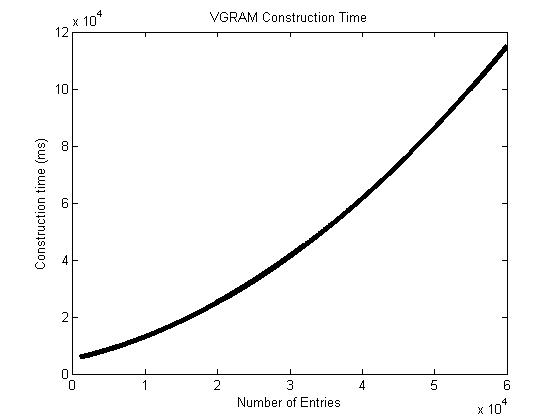
\includegraphics[width=\textwidth]{VGRAMconstructionTime.jpg}
\label{fig:vgram}
\end{subfigure}
\begin{subfigure}[b]{0.45\textwidth}
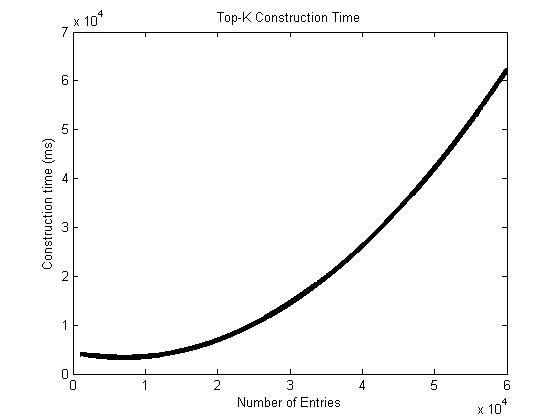
\includegraphics[width=\textwidth]{TOPKconstructionTime.jpg}
\label{fig:topk}
\end{subfigure}
\begin{center}
Figure 1: Construction times for VGRAM and Top-K per data set sizes.
\end{center}
\end{figure}

\subsection{Query executions}
\begin{figure}[h!]
\centering
\begin{subfigure}[b]{0.45\textwidth}
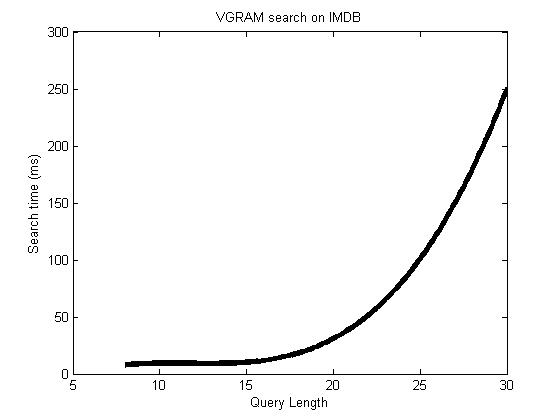
\includegraphics[width=\textwidth]{VGRAMonIMDB.jpg}
\label{fig:imdb}
\end{subfigure}
\begin{subfigure}[b]{0.45\textwidth}
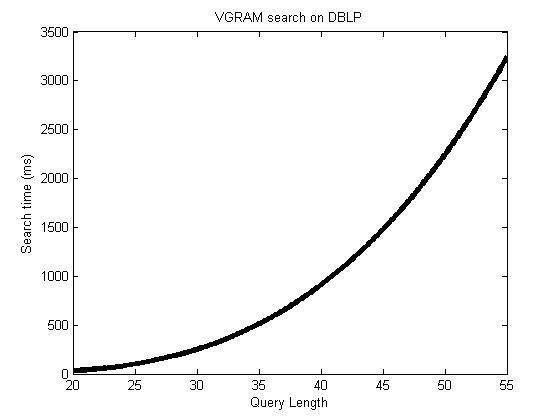
\includegraphics[width=\textwidth]{VGRAMonDBLP.jpg}
\label{fig:dblp}
\end{subfigure}
\begin{center}
Figure 2: Query times per IMDB and DBLP data sets using the VGRAM Trie.
\end{center}
\end{figure}

\begin{figure}[h!]
\centering
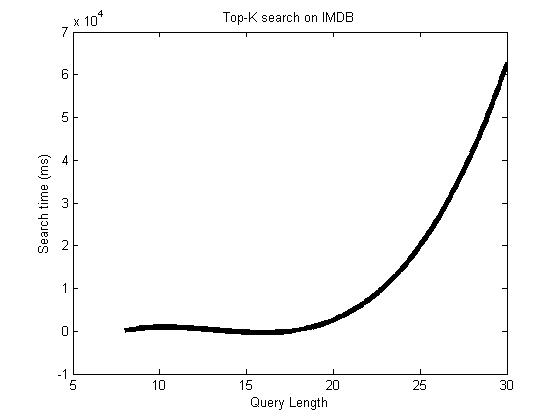
\includegraphics[width=0.5\textwidth]{TOPKonIMDB.jpg}
\begin{center}
Figure 3: Query times for IMDB data set using the Top-K Trie. The full DBLP data set was too large for Top-K queries.
\end{center}
\end{figure}

\newpage
\section{Conclusions}
In this paper, we presented a pruning technique that relies on common data mining and indexing techniques

\section{References}
\begin{enumerate}
\item Don Deng, Guoliang Li, Jianhua Feng, Wen-Syan Li, Top-\textit{k} String Similarity Search with Edit-Distance Constraints, ICDE 2013.
\item C. Li, B. Wang, X, Yang. VGRAM: Improving Performance of Approximate Queries on String Collections Using Variable-Length Grams. VLDB, September 23-27, 2007.
\item M. Hadjieleftheriou, N. Koudas, and D. Srivastava. Incremental maintenance of length normalized indexes for approximate string matching. \textit{SIGMOD Conference}, pages 429-440, 2009.
\item A. Andoni and K. Onak. Approximating edit distance in near-linear time. STOC, pages 199-204, 2009.
\item W. J. Masek and M. Paterson. A faster algorithm computing string edit distances. \textit{Journal of Computer and System Sciences}, 20(1):18-31, 1980.
\item T. Kahveci and A. K. Singh. Efficient index structures for string databases. VLDB, pages 351-360, 2001.
\item Z. Yang, J. Yu and M. Kitsuregawa. Fast algorithms for top-\textit{k} approximate string matching. AAAI, 2010.
\item R. Zafarani and H. Liu. Connecting users across social media sites: a behavioral-modeling approach. KDD, pages 41-49, 2013.
\end{enumerate}

\FloatBarrier
\end{document}